\documentclass{beamer}

\input{../../preamble/slidespreamble.tex}

\usepackage{amsfonts}
\usepackage{tikz}

\parskip=0.5em

\title{Scientific Computing for Biologists}
\subtitle{Lecture 7 \\
        Testing for Group Effects and Contrasting Groups:\\
         ANOVA and Discriminant Analysis}

\author{Instructor: Paul M. Magwene}
\date{09 October 2012}


\begin{document}

%===========================================================
\begin{frame}
\titlepage
\end{frame}
%===========================================================


%===========================================================
\begin{frame}
  \frametitle{Outline of Lecture}

\begin{itemize}
    \item ANOVA as multiple regression
    \item Fisher's Discriminant Function
    \item Canonical Variates Analysis (CVA)
    \begin{itemize}
        \item Geometric and Algebraic View
        \item Similarities and differences between CVA and PCA
        \item Interpretting CVA
    \end{itemize}

\end{itemize}

\end{frame}
%===========================================================



%===========================================================
\begin{frame}[fragile]
  \frametitle{Testing the Regression Effects}

\begin{figure}
{\centering \includegraphics[height=1.5in]{fig-multireg.pdf}}
\caption{Geometry of multiple regression.}
\end{figure}
%
\begin{align*}
|\vec{y}|^2 &= SS_{\text{total}} \\
|\vec{\hat{y}}|^2 &= SS_{\text{regression}} = R^2 SS_{\text{total}}\\
|\vec{d}|^2 &= SS_{\text{resiudal}}  = (1-R^2)SS_{\text{total}}
\end{align*}
%
\begin{center}
\alert{Is my regression significant? $\implies$ Is $|\vec{\hat{y}}|^2$ large relative to $|\vec{e}|^2$?}
\end{center}

\end{frame}
%===========================================================

%===========================================================
\begin{frame}
  \frametitle{Geometry of the Population Regression Model}


\begin{figure}
{\centering \includegraphics[height=2in]{regr-error-model2.pdf}}
\caption{\textbf{Left:} null hypothesis of no regression effects is true; \textbf{Right:} null model is false.}
\end{figure}

\begin{center}
\alert{Null Hypothesis: }  $H_0: \beta_1 = \beta_2 = \cdots = \beta_p = 0$
\end{center}

\end{frame}
%===========================================================


%===========================================================
\begin{frame}
  \frametitle{Dimensionality of Regression Subspaces}


\begin{figure}
{\centering \includegraphics[height=2in]{regr-dimofspaces.pdf}}
\end{figure}
%
\begin{align*}
  \dim(\mathcal{V}_\text{total}) & = N &\text{(total)}\\
  \dim(\mathcal{V}_1) & = 1 &\text{(mean effect)} \\
  \dim(\mathcal{V}_x) & = p &\text{(effect space)}\\
  \dim(\mathcal{V}_e) & = N - p - 1 &\text{(error space)}
\end{align*}

\end{frame}
%===========================================================


%===========================================================
\begin{frame}
  \frametitle{Comparing the Effect Space and the Error Space}

To compare the squared length of $|\vec{\hat{y}}|^2$ and $|\vec{e}|^2$ we divide them by the dimension of the subspaces in which they lie.
\begin{align*}
M(\vec{\hat{y}}) &= \frac{|\vec{\hat{y}}|^2} {\dim(\mathcal{V}_x)}   \\
M(\vec{e})       &= \frac{|\vec{e}|^2}{\dim(\mathcal{V}_e)}
\end{align*}

We compare these by defining a statistic, $F$:
\begin{align*}
  F = \frac{M(\vec{\hat{y}})}{M(\vec{e})} &= \frac{\dim(\mathcal{V}_e)|\vec{\hat{y}}|^2}
                                                  {\dim(\mathcal{V}_x)|\vec{e}|^2}\\
 &= \frac{(N-p-1)R^2}{p(1-R^2)}
\end{align*}

\alert{When null hypothesis is true, $F\approx 1$; when it is false, $F \gg 1$.}

\end{frame}
%===========================================================



%===========================================================
\begin{frame}
  \frametitle{Two-group ANOVA as Regression}

We can also use a geometric perspective to test whether the mean of a variable differs between two groups of subjects.

\begin{itemize}
\item Setup a `dummy variable' as the predictor $X_g$.   We assign all subjects in group 1 the value 1 and all subjects in group 2 the value -1 on the dummy variable.  We then regress the variable of interest, $Y$, on $X_g$.

\end{itemize}
%
$$
\Mtx{y} = \Mtx{X}_g\Mtx{b} + \Mtx{e}
$$
%
\begin{figure}
{\centering \includegraphics[height=1.5in]{anova-2group-table.pdf}}
\end{figure}


\end{frame}
%===========================================================


%===========================================================
\begin{frame}
  \frametitle{Two-group ANOVA as Regression, cont}

\begin{itemize}

\item When the means are different in the two groups, $X_g$ will be a good predictor of the variable of interest, hence $\vec{y}$ and $\vec{x_g}$ will have a small angle between them.

\item When the means in the two groups are similar, the dummy variable will not be a good predictor.  Hence the angle between $\vec{y}$ and $\vec{x_g}$ will be large.

\end{itemize}

\begin{center}

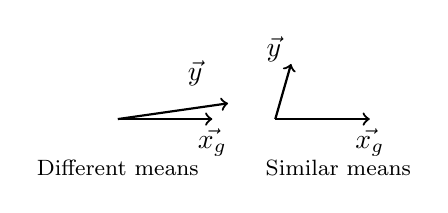
\begin{tikzpicture}[x=0.2cm, y=0.2cm]

% different means
\draw[thick,->] (-10,0) -- (-4,0);
\draw (-4,0) node[below] {$\vec{x_g}$};

\draw[thick,->] (-10,0) -- (-3,1);
\draw (-4,1.5) node[above left] {$\vec{y}$};
\draw (-10,-2) node[below,font=\footnotesize] {Different means};

% Similar means
\draw[thick,->] (0,0) -- (6,0);
\draw (6,0) node[below] {$\vec{x_g}$};

\draw[thick,->] (0,0) -- (1,3.5);
\draw (1,3) node[above left] {$\vec{y}$};
\draw (4,-2) node[below,font=\footnotesize] {Similar means};

\end{tikzpicture}

\end{center}

\end{frame}
%===========================================================

%===========================================================
\begin{frame}
  \frametitle{Multi-way ANOVA as Regression}

\begin{itemize}

\item Exactly the same idea applies to $g$ groups, except now instead of one grouping variable, we define $g-1$ grouping variables, $\dim(X_g) = g-1$.

\item Then we calculate the multiple regression as we did before:

\end{itemize}

$$
\Mtx{y} = \Mtx{X}\Mtx{b} + \Mtx{e}
$$

$$
\Mtx{y} = \left[ \begin{array}{c}
y_1 \\ y_2 \\ \vdots \\y_n \\
\end{array}
\right]
\;
;
\;
\Mtx{X} = \left[ \begin{array}{ccccc}
1 & x_{11} & x_{12} & \cdots & x_{1g} \\
1 & x_{21} & x_{22} & \cdots & x_{2g} \\
\vdots & \vdots & \vdots & \vdots & \vdots \\
1 & x_{n1} & x_{n2} & \cdots & x_{ng} \\
\end{array}
\right]
\;
;
$$
%
Estimate \Mtx{b} as:
$$
\Mtx{b} = (\Mtx{X}^T \Mtx{X})^{-1}\Mtx{X}^T\Mtx{y}
$$

\end{frame}
%===========================================================

%===========================================================
\begin{frame}
  \frametitle{How Do We Construct the Grouping Matrix, $X_g$?}

Two common methods are:

\begin{enumerate}
\item Dummy coding -- define a set of $g$ grouping variables, where values take either 0 or 1, depending on group membership, but \emph{use only the first} $g-1$ columns:
%
\begin{equation*}
U_j = \left\{
\begin{aligned}
1, &\qquad \text{for every subject in group } j, \\
0, &\qquad \text{for all other subjects.}
\end{aligned}
\right.
\end{equation*}
and
%
$$
X_g= [U_1, U_2, \cdots, U_{g-1}]
$$
%
\item Effect coding -- define the $U_j$ as above, and set:
$$
X_g = [U_1 - U_g, U_2-U_g, \cdots, U_{g-1} - U_g]
$$
\end{enumerate}

In general, effect coding is more similar to standard ANOVA contrasts.

\end{frame}
%===========================================================


%===========================================================
\begin{frame}[fragile]
  \frametitle{ANOVA: Example Data Set}
\small
\begin{center}
\begin{tabular}{lrrrrr}
  \toprule
  & $g_1$ & $g_2$ & $g_3$ & $g_4$ \\
  \midrule
  & 20 & 21 & 17 & 8 & \\
  & 17 & 16 & 16 & 11 &  \\
  & 17 & 14 & 15 & 8 & \\
  \midrule
$M_{g.}$ & 18& 17 & 16 & 9 & $M_{..}=15$ \\
\bottomrule
\end{tabular}
\end{center}
%
\footnotesize
\begin{equation*}
y = \begin{bmatrix}
20 \\ 17 \\ 17 \\
21 \\ 16 \\ 14 \\
17 \\ 16 \\ 15 \\
8 \\ 11 \\ 8
\end{bmatrix}
,\qquad
\Mtx{X} = \begin{bmatrix}
1 & 1 & 0 & 0 \\
1 & 1 & 0 & 0 \\
1 & 1 & 0 & 0 \\
1 & 0 & 1 & 0 \\
1 & 0 & 1 & 0 \\
1 & 0 & 1 & 0 \\
1 & 0 & 0 & 1 \\
1 & 0 & 0 & 1 \\
1 & 0 & 0 & 1 \\
1 & -1 & -1 & -1 \\
1 & -1 & -1 & -1 \\
1 & -1 & -1 & -1
\end{bmatrix}
\end{equation*}
\end{frame}
%===========================================================

%===========================================================
\begin{frame}[fragile]
  \frametitle{ANOVA: Example Data Set, cont}
\small

Solving for $\Mtx{b}$ we find:

\begin{equation*}
\Mtx{b} = \begin{bmatrix}
15 \\ 3 \\ 2 \\ 1
\end{bmatrix},
\; \quad |\hat{\Mtx{y}}|^2 = 150, \;|\Mtx{e}|^2 = 40
\end{equation*}
Since, $\dim(\mathcal{V}_x) = 3$, and $\dim(\mathcal{V}_e)= 8$,  we get:
\begin{equation*}
  F = \frac{\dim(\mathcal{V}_e)|\vec{\hat{y}}|^2}
              {\dim(\mathcal{V}_x)|\vec{e}|^2}
    = 10
\end{equation*}

Here's the more conventional ANOVA table for the same data:
\footnotesize
\begin{center}
\begin{tabular}{lrrrrr}
  \toprule
 Source & df & $SS$ & $MS$ & $F$ & $\Pr(F)$ \\
  \midrule
 Experimental  & 3 & 150 & 50 & 10 & .0044\\
 Error  & 8  & 40 & 5 & \\
 \midrule
 Total & 11 & 190 & &\\
\bottomrule
\end{tabular}
\end{center}


\end{frame}
%===========================================================



%===========================================================
\begin{frame}
  \frametitle{Overview of Discriminant Analysis}

\begin{block}{Discrimination}
Given an $n \times p$ data matrix, \Mtx{X}, and a grouping of the $n$ specimens into $g$ groups, find the linear combination of the variables, $\Mtx{a}'\Mtx{x}$ that best discriminates between the groups (using $'$ to indicate transpose).
\end{block}

\begin{block}{Classification}
Given $g$ groups, define a function that assigns an object with unknown assignment to the `best' group.
\end{block}


\end{frame}
%===========================================================


%===========================================================
\begin{frame}
  \frametitle{Fisher's Discriminant Function}

\begin{itemize}
\item Applies to the two-group case.
\item Solution: find \Mtx{a} that maximizes the ratio of the squared group mean difference to within-group variance:
\end{itemize}

\[
F = \frac{(\Mtx{a}'\bar{\Mtx{x}}_1 - \Mtx{a}'\bar{\Mtx{x}}_2)^2}{\Mtx{a}'\Mtx{W}\Mtx{a}}
\]

where
\begin{itemize}
\item $\bar{\Mtx{x}}_1 = \frac{1}{n_1}\sum_{i=1}^{n_1} \Mtx{x}_{1i}$
\item $\bar{\Mtx{x}}_2 = \frac{1}{n_2}\sum_{i=1}^{n_2} \Mtx{x}_{2i}$
\item $\Mtx{W} = \frac{1}{n_1 + n_2 - 2}\sum_{i=1}^{2}\sum_{j=1}^{n_i}(\Mtx{x}_{ij} - \bar{\Mtx{x}}_i)(\Mtx{x}_{ij} - \bar{\Mtx{x}}_i)'$ (w/in-group pooled covariance matrix)
\item $n_i$ indicates the number of observations in the $i$th group and the $\Mtx{x}_{i1},\ldots,\Mtx{x}_{in_i}$ represent the specific observations (as vectors).
\end{itemize}

% Given an $n \times p$ data matrix, \Mtx{X}, and a grouping of the $n$ specimens into $g$ groups, find the linear coeffients, \Mtx{a}, such that  of the variables, $\Mtx{a}\Mtx{x}_i$ that best discriminates between the groups.
% \end{block}
%
% Solution: find a that maximizes the ratio of the squared group mean difference to within-group variance:
%
%
%

\end{frame}
%===========================================================

%===========================================================

\begin{frame}
  \frametitle{Geometry of the Two-Group Discriminant Function}

\begin{center}
\includegraphics[height=3.1in]{2group}
\end{center}

\end{frame}
%===========================================================

%===========================================================
\begin{frame}
  \frametitle{Fisher's LDF}


\[
F = \frac{(\Mtx{a}'\bar{\Mtx{x}}_1 - \Mtx{a}'\bar{\Mtx{x}}_2)^2}{\Mtx{a}'\Mtx{W}\Mtx{a}}
\]


Maximizing $F$ gives:

\[
\Mtx{a} = c\Mtx{W}^{-1}(\bar{\Mtx{x}}_1 - \bar{\Mtx{x}}_2)
\]

where $c$ is an arbitrary constant (usually taken to be 1).

\end{frame}
%===========================================================


%===========================================================
\begin{frame}
  \frametitle{Fisher's LDF as Classification}

Fisher's solution can also be setup as a classification solution using regression.

\begin{itemize}
\item setup a dummy variable, $\Mtx{y}$ that takes the values:
\begin{itemize}
    \item $y_1 = n_2/(n_1 + n_2)$ for observations in group 1
    \item $y_2 = -n_1/(n_1 + n_2)$ for observations in group 2
\end{itemize}
\item Solve the standard multivariate regression, $\Mtx{y} = \Mtx{X}\Mtx{b} + \Mtx{e}$
\item Allocate unknown individual to group 1 if it's predicted $y$ is closer to $y_1$ than to $y_2$, otherwise assign to group 2.

\end{itemize}

%% What is the subspace of X, that is closest to the y_g (the grouping variable) -- i.e. regressing grouping variable on continuous X (rather than regressing continuous y on grouping variable X in ANOVA case)

\end{frame}
%===========================================================

%===========================================================
\begin{frame}
  \frametitle{What if there are more than two groups?}

The multi-group equivalent of Fisher's LDF is called `Canonical Variate Analysis' (CVA).

\begin{itemize}
\item straight forward extension of Fisher's solution
\item Find \Mtx{a} that maximizes the ratio of between-group to within-group variance:

\[
F = \frac{\Mtx{a}'\Mtx{B}\Mtx{a}}{\Mtx{a}'\Mtx{W}\Mtx{a}}
\]

\item \Mtx{W} is within-group matrix (as defined previously)
\item \Mtx{B} is the between-group covariance matrix
\begin{itemize}
    \item $\Mtx{B}_w = \frac{1}{g-1}\sum_{i=1}^{g} n_i(\Mtx{x}_i - \bar{\Mtx{x}})(\Mtx{x}_i - \bar{\Mtx{x}})'$ where $n_i$ is the sample size in group $i$ (weighted version)
    \item  $\Mtx{B}_u = \frac{1}{g-1}\sum_{i=1}^{g} (\Mtx{x}_i - \bar{\Mtx{x}})(\Mtx{x}_i - \bar{\Mtx{x}})'$ (unweighted version)
\end{itemize}

\end{itemize}



\end{frame}
%===========================================================

%===========================================================
\begin{frame}
  \frametitle{Geometry of CVA}

\begin{center}
\includegraphics[height=3.1in]{3group}
\end{center}

\end{frame}
%===========================================================


%===========================================================
\begin{frame}
  \frametitle{CVA Solution}

Maximizing $F$ leads to the following:
\[
(\Mtx{B} - l\Mtx{W})\Mtx{a} = \Mtx{0}
\]

\begin{itemize}
\item $l$ is an eigenvalue of $\Mtx{W}^{-1}\Mtx{B}$
\item $\Mtx{a}$ is an eigenvector of $\Mtx{W}^{-1}\Mtx{B}$
\end{itemize}

There will be $s=\min(p, g-1)$ non-zero eigenvalues.
\medskip

Organize the eigenvectors, $\Mtx{a}_i$, as columns of a $p \times s $ matrix \Mtx{A}.
\begin{itemize}
\item The \textbf{\emph{canonical variates}} are given by $\Mtx{y} = \Mtx{A}'\Mtx{x}$
\item The mean of the $i$-th group in the canonical variates space is given by $\bar{\Mtx{y}}_i = \Mtx{A}'\bar{\Mtx{x}}_i$
\end{itemize}

\end{frame}
%===========================================================

%===========================================================
\begin{frame}
  \frametitle{CVA as a two-stage rotation I}

\begin{center}
\includegraphics[width=\textwidth]{cva-as-rot1}
\end{center}

\hfill {\scriptsize \textit{From MacLeod 2010, PalaeoMath newsletter}}

\end{frame}
%===========================================================

%===========================================================
\begin{frame}
  \frametitle{CVA as a two-stage rotation II}

\begin{center}
\includegraphics[width=0.9\textwidth]{cva-as-rot2}
\end{center}

\hfill {\scriptsize \textit{From MacLeod 2010, PalaeoMath newsletter}}


\end{frame}
%===========================================================

%===========================================================
\begin{frame}
  \frametitle{CVA as a two-stage rotation III}

\begin{center}
\includegraphics[width=0.9\textwidth]{cva-as-rot3}
\end{center}

\hfill {\scriptsize \textit{From MacLeod 2010, PalaeoMath newsletter}}


\end{frame}
%===========================================================

%===========================================================
\begin{frame}
  \frametitle{CVA as a two-stage rotation IV}

\begin{center}
\includegraphics[width=\textwidth]{cva-as-rot4}
\end{center}

\hfill {\scriptsize \textit{From MacLeod 2010, PalaeoMath newsletter}}

\end{frame}
%===========================================================


%===========================================================
\begin{frame}
  \frametitle{Similarities and Differences between CVA and PCA}

PCA:
\begin{itemize}
\item Uncorrelated over the whole sample
\item orthogonal transformation from the original variates, \Mtx{x}, to the new variates \Mtx{y}. PC axes at right angles to each other in the space of the original variables.
\end{itemize}

CVA:
\begin{itemize}
\item Canonical variates are uncorrelated both \emph{within} and \emph{between} groups
\item Canonical variates have equal variance \emph{within} groups, but in decreasing order \emph{between} groups
\item non-orthogonal transformation, CV axes \emph{not} at right angle to each other in the original frame of reference.
\end{itemize}
\end{frame}

%===========================================================
%@nonl
%@-node:pmagwene.20061107103153:Similarities/Differences w/PCA
%@+node:pmagwene.20061107110604:Illustration of PCA vs CVA


%===========================================================
\begin{frame}
  \frametitle{PCA vs CVA: A Motivating Example}

\begin{center}
\includegraphics[height=2.5in]{simple2group}

What is the direction of PC1? What is the direction of CVI?
\end{center}

\end{frame}
%===========================================================

% %===========================================================
% \begin{frame}
%   \frametitle{The different components of interest}
%
% \begin{center}
% \includegraphics[height=3in]{krz-components}
% \end{center}
%
% \end{frame}
% %===========================================================


%===========================================================
\begin{frame}
  \frametitle{PCA vs. CVA: Anderson's Iris Data}

\begin{columns}

\begin{column}{0.5\textwidth}
\begin{center}
\includegraphics[width=\textwidth]{iris-PCA}
\end{center}
\end{column}

\begin{column}{0.5\textwidth}
\begin{center}
\includegraphics[width=\textwidth]{iris-CVA}
\end{center}
\end{column}

\end{columns}
\end{frame}
%===========================================================

% %===========================================================
% \begin{frame}
%   \frametitle{Mahalanobis Distance I}
%
% \begin{block}{Question}
% If canonical variates are not orthogonal, what justifies plotting them as so?
% \end{block}
%
% \begin{block}{Answer}
% A consideration of multivariate distance is the justification for orthogonal representation of CVs.
% \end{block}
%
%
% \end{frame}
% %===========================================================
%
% %===========================================================
% \begin{frame}
%   \frametitle{Mahalanobis Distance II}
%
% Consider:
% \begin{itemize}
% \item if all variates have equal variances and are uncorrelated w/in groups than Euclidean distance between group means is an accurate representation of (statistical) dissimilarity
% \item However, if some variables have very large variance or pairs of variables are highly correlated than Euclidean distance between group means isn't a good representation of the `true' dissimilarity in terms of variational trends
% \end{itemize}
%
% see illustration on board.
%
% \end{frame}
% %===========================================================
%
% %===========================================================
% \begin{frame}
%   \frametitle{Mahalanobis Distance III}
%
% A dissimilarity measure that takes into account patterns of variance/covariance is called `Mahalanobis Distance'.
%
% The Mahalanobis distance between the $i$th and $j$th group means is given by:
% \[
% D^2 = (\bar{\Mtx{x}}_i - \bar{\Mtx{x}}_j)' \Mtx{W}^{-1} (\bar{\Mtx{x}}_i - \bar{\Mtx{x}}_j)
% \]
%
% It turns out that by constructing orthogonal axes from the canonical variates than Euclidean distance in the canonical variate space corresponds  (approximately) to Mahalanobis distance in the original variate space.
%
% \emph{Sidenote} -- The distance between the individual point $\Mtx{x}_i$ and the mean of a $\bar{\Mtx{x}}$ of a single sample is given by $d^2 = (\Mtx{x}_i - \bar{\Mtx{x}})' S^{-1} (\Mtx{x}_i - \bar{\Mtx{x}})$ where \Mtx{S} is the covariance matrix.
%
% \end{frame}
% %===========================================================

%===========================================================
\begin{frame}
  \frametitle{Are any of the groups significantly different in the canonical variate space?}

To test:
\begin{itemize}
\item $H_0: \mu_1 = \mu_2 = \ldots = \mu_3$
\item $H_1$: at least one $\mu_i$ differs from the rest
\end{itemize}

A couple of approaches:
\begin{itemize}
\item  Compare the largest eigenvalue, $l_1$, of $\Mtx{W}^{-1}\Mtx{B}$ to critical values in a F-table. $H_0$ is rejected for large values ($>1$).
\item Likelihood approach:
\begin{itemize}
\item Wilks' lambda, $\Lambda = |\Mtx{W}|/|\Mtx{B} + \Mtx{W}| = \prod_{i=1}^{p} (1 + l_i)^{-1}$
\item there is an approximation that has a $\chi^2$ distribution.
\end{itemize}
\end{itemize}

Both boil down to a consideration of eigenvalues of $\Mtx{W}^{-1}\Mtx{B}$.

\end{frame}
%===========================================================


%===========================================================
\begin{frame}
  \frametitle{Which groups are different? Where does an unassigned observation belong?}

Within groups the canonical variates are:
\begin{itemize}
\item uncorrelated
\item have unit variance
\end{itemize}

If we assume multivariate normality of the data then we can exploit this to draw confidence intervals around the group means in the canonical variate space.
\smallskip

A 100(1-$\alpha$) percent confidence region for the true mean $\Mtx{v}_i$ is given by:
\begin{itemize}
\item hypersphere centered at $\bar{\Mtx{y}}_i$
\item with radius ($\chi^{2}_{\alpha,r}/n_i)^{1/2}$ where $r$ is the number of canonical variate dimensions considered
\end{itemize}

\end{frame}
%===========================================================


%===========================================================
\begin{frame}
  \frametitle{Illustration of group means and tolerance regions}

\begin{center}
\includegraphics[height=3.1in]{iris-CVA-meantol}
\end{center}

\end{frame}
%===========================================================


%===========================================================
\begin{frame}
  \frametitle{Which variables are most important in CVA?}

\begin{block}{Question}
Which variables are most `important' in distinguishing between the groups?
\end{block}

Consider the coefficients $\Mtx{a}_i$
\begin{itemize}
\item large coefficients may be due to \emph{either} large between-group variability \emph{or} small within-group variability of the corresponding variable
\item for interpretation it's better to consider modified coefficient, $\Mtx{a}_{i}^{*} = (a_{i1}^{*},\ldots,a_{ip}^{*})$ where the $a_{ij}^{*}$ are given by $a_{ij}^{*} = a_{ij}\sqrt{w_{jj}}$ [$w_{jj}$ are the diagonal elements of \Mtx{W}].
\end{itemize}

\end{frame}
%===========================================================


% %===========================================================
% \begin{frame}
%   \frametitle{CVA as a two-step PCA}
%
% \begin{center}
% \includegraphics[height=3.2in]{two-step-cva}
% \end{center}
%
% \end{frame}
% %===========================================================


\end{document}
